\section{Introduction}
\label{sec-introduction}

Two trends are combining to create increasingly crowded and uncoordinated
home \wifi{} environments. First, increasing broadband penetration is
creating larger numbers of private home access points (APs). Strategy
Analytics estimated that by the end of 2014, 451~M households worldwide
(25\%) would have home \wifi{} and that this number will continue to
grow~\cite{wifi-survey}. Second, an increasing percentage of the world's
population resides in dense urban environments: 54\% today and climbing to
66\% by 2050~\cite{urbanization-survey}. Together these two trends create a
future where more people will operate private home APs that overlap with
other nearby private home APs.

\begin{figure}[t]
  %
  \centering
  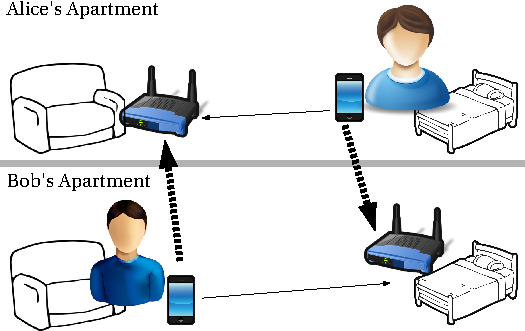
\includegraphics[width=0.9\columnwidth]{./figures/motivation.pdf}
  %
  %\vspace*{-0.1in}
  %
  \caption{\textbf{Example of Reciprocal \wifi{} Sharing.} Solid arrows
  represent weak connections, while dashed lines represent strong
  connections.}
  %
  \label{fig:motivation}
  %
  \vspace*{-0.1in}
\end{figure}

Unfortunately, uncoordinated deployment of overlapping private networks can
create interference that degrades performance, which may then cause users to
respond in ways that further exacerbate the problem. Consider Alice's/Bob's
apartment shown in Figure~\ref{fig:motivation}. Alice/Bob has deployed
her/his AP in her/his living room/bedroom. Due to the proximity of their
apartments, Alice/Bob receives a stronger signal from Bob's/Alice's router
when she/he is in her/his bedroom/living room. But because Alice/Bob cannot
connect to Bob's/Alice's router, she/he must either use the lower-bandwidth
connection to her/his existing AP or deploy an additional AP in her/his
bedroom/living room. Both options generate additional wireless interference
for her/his neighbors, including Bob/Alice.

Ideally, Alice/Bob would allow Bob/Alice to use her/his router. Obviously
this solution requires less hardware. But it also improves performance while
reducing interference and client energy consumption, both by allowing the APs
to coordinate overlapping transmissions and by allowing clients to achieve
higher bitrates at lower transmission powers. We refer to this
mutually-beneficial arrangement as \textit{reciprocal \wifi{} sharing}.

Reciprocal \wifi{} sharing has benefits compared to attempts to use private
APs to establish community networks such as FON~\cite{fon} or
OpenWireless~\cite{openwireless}. Reciprocal \wifi{} sharing opportunities
are more likely to align with existing human relationships, such as this
example involving two neighbors, rather than requiring users to open their
private networks to strangers. And because reciprocal \wifi{} sharing
involves only pairwise cooperation, agreements can be established and
monitored without the elaborate reputation systems or credit mechanisms
required to prevent freeloading in large communities. Once Alice notices that
the sharing agreement with Bob is no longer beneficial---either because she
no longer needs his connection or because he is degrading her service to the
point where it is no longer useful---she can immediately terminate it.

But how often is reciprocal \wifi{} sharing beneficial and possible in
practice? To explore these questions, we begin in
Section~\ref{sec:investigation} by analyzing a dataset collected on the
\PhoneLab{}~smartphone testbed containing \num{21192417} \wifi{} scan results
from 254~smartphones over 5~months. Despite the
fact that the geographic extent of the dataset is suburban Buffalo, which as
a city has a population density an order of magnitude lower than
densely-populated areas like Manhattan, we still find that many users would
benefit from being able to connect to neighboring private networks. Even more
surprisingly, despite monitoring only several hundred users we were still
able to observe reciprocal \wifi{} sharing opportunities in our tiny
sample. Motivated by these results Section~\ref{sec:design} presents the
design of \wisefi{}, a system addressing the practical challenges of
establishing and monitoring reciprocal \wifi{} sharing agreements. We
conclude by identifying some open challenges in implementing such a system as
future work in Section~\ref{sec:challenges}.
